\documentclass[../../main.tex]{subfiles}
\begin{document}

\begin{flushright}
\footnotesize\textit{【自動文字起こし・要確認】}
\end{flushright}

{\bf [解]}
グラフは下図である．
\begin{align*}
\frac34x^2-5=x\quad&\cdots①\ \text{の2解}\ \alpha,\beta\ (\alpha<\beta)\\
-\frac34x^2+1=x\quad&\cdots②\ \text{の2解}\ \gamma,\delta\ (\gamma<\delta)
\end{align*}
とおく．もとめる面積を$S$とする．

\begin{figure}[htb]
\centering
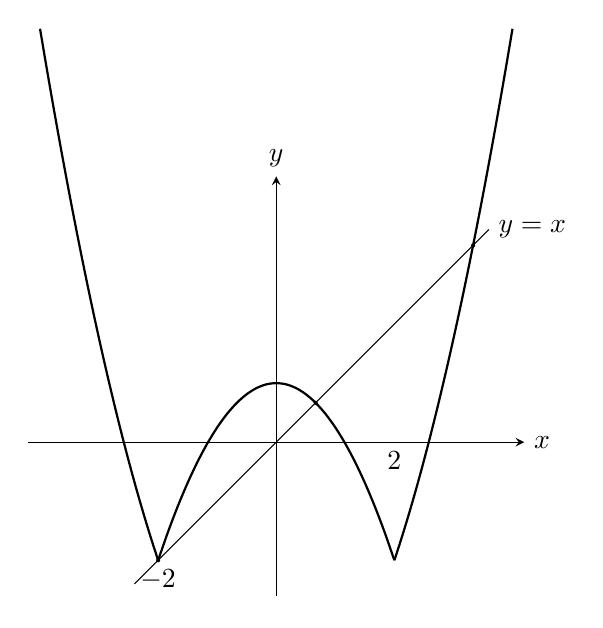
\begin{tikzpicture}[scale=0.75, >=stealth]
  \draw[->] (-4.2,0) -- (4.2,0) node[right] {$x$};
  \draw[->] (0,-2.6) -- (0,4.5) node[above] {$y$};
  \draw[domain=-4:-2, smooth, thick] plot (\x,{0.75*\x*\x-5});
  \draw[domain=-2:2, smooth, thick] plot (\x,{-0.75*\x*\x+1});
  \draw[domain=2:4, smooth, thick] plot (\x,{0.75*\x*\x-5});
  \draw[domain=-2.4:3.6, smooth] plot (\x,{\x}) node[right] {$y=x$};
  \node[below] at (-2,-2) {$-2$};
  \node[below] at (2,0) {$2$};
  \fill (-2,-2) circle (1pt);
  \fill (0.667,0.667) circle (1pt);
  \fill (3.333,3.333) circle (1pt);
\end{tikzpicture}
\caption{$y=x$と$y=\left|\frac34x^2-3\right|-2$で囲まれる部分（斜線部）}
\end{figure}

\begin{align*}
S=(\text{①を全区間で延長した放物線と直線の間の面積})+2\times(\text{②の放物線と直線の間の面積})\\
-2\times(\text{①を延長した放物線と直線の間の，区間}[-2,2]\text{での面積})\quad\cdots③
\end{align*}

であり，
\begin{align*}
&\frac34\cdot\frac16(\beta-\alpha)^3=\frac18(\beta-\alpha)^3，\\
&\frac34\cdot\frac16(\delta-\gamma)^3=\frac18(\delta-\gamma)^3，\\
&\frac34\cdot\frac16(2+2)^3=\frac18(4)^3
\end{align*}

を③に代入して
\begin{align*}
S=\frac18(\beta-\alpha)^3+\frac14(\delta-\gamma)^3-16\quad\cdots④
\end{align*}

ここで，①，②から
\begin{align*}
\beta-\alpha=\frac{10}3+2=\frac{16}3，\qquad\delta-\gamma=\frac23+2=\frac83
\end{align*}

を④に代入して
\begin{align*}
S&=\frac18\left(\frac{16}3\right)^3+\frac14\left(\frac83\right)^3-16\\
&=\frac{8^3}{3^3}+\frac{2\cdot8^2}{3^3}-\frac{16\cdot3^3}{3^3}\\
&=\frac{16}{3^3}(32+8-27)\\
&=\frac{208}{27}．
\end{align*}

\newpage

\end{document}
